\chapter{Monte Carlo corrections}
Monte Carlo plays important role in cross-section measurement. It is constantly undergoing correction to data, in order to obtain a required precision. Part of this corrections have been described in a chapter \ref{chap:MC}. Unfortunatelly,  not everything can be taken into account during simulation itself. This leads to a differences between data and monte carlo, that needs to be accounted for. There are two possible methods to correct monte carlo without regenerating it. First on is to apply event weight, so what each mc event can contribute to non 1 entries in a histogram.This is called reweighting. Second one is to smear MC. It is using random number to alter reconstructed 4-vectors. 
This chapter describes all additional corrections, what have been applied on MC in this analysis. All of this correction are introducing additional systematic error, that will be discussed in the chapter \ref{sec:}
\section{Number of vertexes reweighting}
The effect of multiple particle interactions per bunch crossing is accounted in MC. But there is sill remaining difference between simulation and collected data. This mismodelling can affect many distributions. One of the ways to correct this is to apply weight on number of vertexes. This variables have a connection between each other, because each pp interaction produces separate vertex. Fig ~\ref{ris:MC_Nvtx} shows a comparison of number of vertexes before and after reweighting.
\section{Lepton efficiency corrections}

Lepton detection efficiency at \atlas detector can be divided into three components:
\begin{itemize}
\item The reconstruction efficiency $\epsilon_{rec}$ is associated to the reconstruction algorithm. It is a probability to reconstruct lepton as a lepton of this flavor .
\item The identification efficiency $\epsilon_{id \mid rec}$ is the probability that a reconstructed lepton survives  identification requirements. 
\item The trigger efficiency $\epsilon_{trig \ mid rec,id}$ is the probability, that lepton satisfiees trigger requirement. 
\end{itemize}
The full efficiency for a single lepton can be written as:
\begin{equation}
\epsilon_{total}=\epsilon_{rec} \times \epsilon_{id \mid rec} \times \epsilon_{trig \mid rec,id}
\end{equation}
All of this efficiencies are measured using Tag and Probe method in $Z\to ll$ decays. This is allowing to insure, that all of the reconstructed lepton candidates are coming from an actual leptons. One of the leptons from Z boson, called "probe", is initially selected with all of the cuts, minus one under study. Second one, called "probe" satisfies more tighter selection with additional cut, such as, for example, trigger matching. 
Simulation samples are corrected to data by a scale-factor :
\begin{equation}
SF_{reco,id,trig}=\frac{\epsilon^{data}_{reco,id,trig}}{\epsilon^{MC}_{reco,id,trig}}
\end{equation}
Each of the scale factors calculated in a $p_{t}$ and $\eta$ bins and has an associated statistical and systematical uncertainty component. Statistical component is connected to a size of $Z\to ll$, which is in our case is around 500 event per each lepton flavor. This means that precise calculation of scaling factors based on this data is difficult.
It is possible to use scale factors for 8 TeV 2012 data. The main difference between this data samples are center of mass energy and a pile-up conditions (10 in 2012 and less than 1 in 2013). This effects have been studied on a $Z\to ee$ sample. Fig. \ref{eff_comp} shows that all of the differences in a scale factors are negligible and fully covered by the statistical error. This justifies the usage of 8 TeV scalling factors with increased uncertainty in this analysis. 

\begin{figure}
\centering
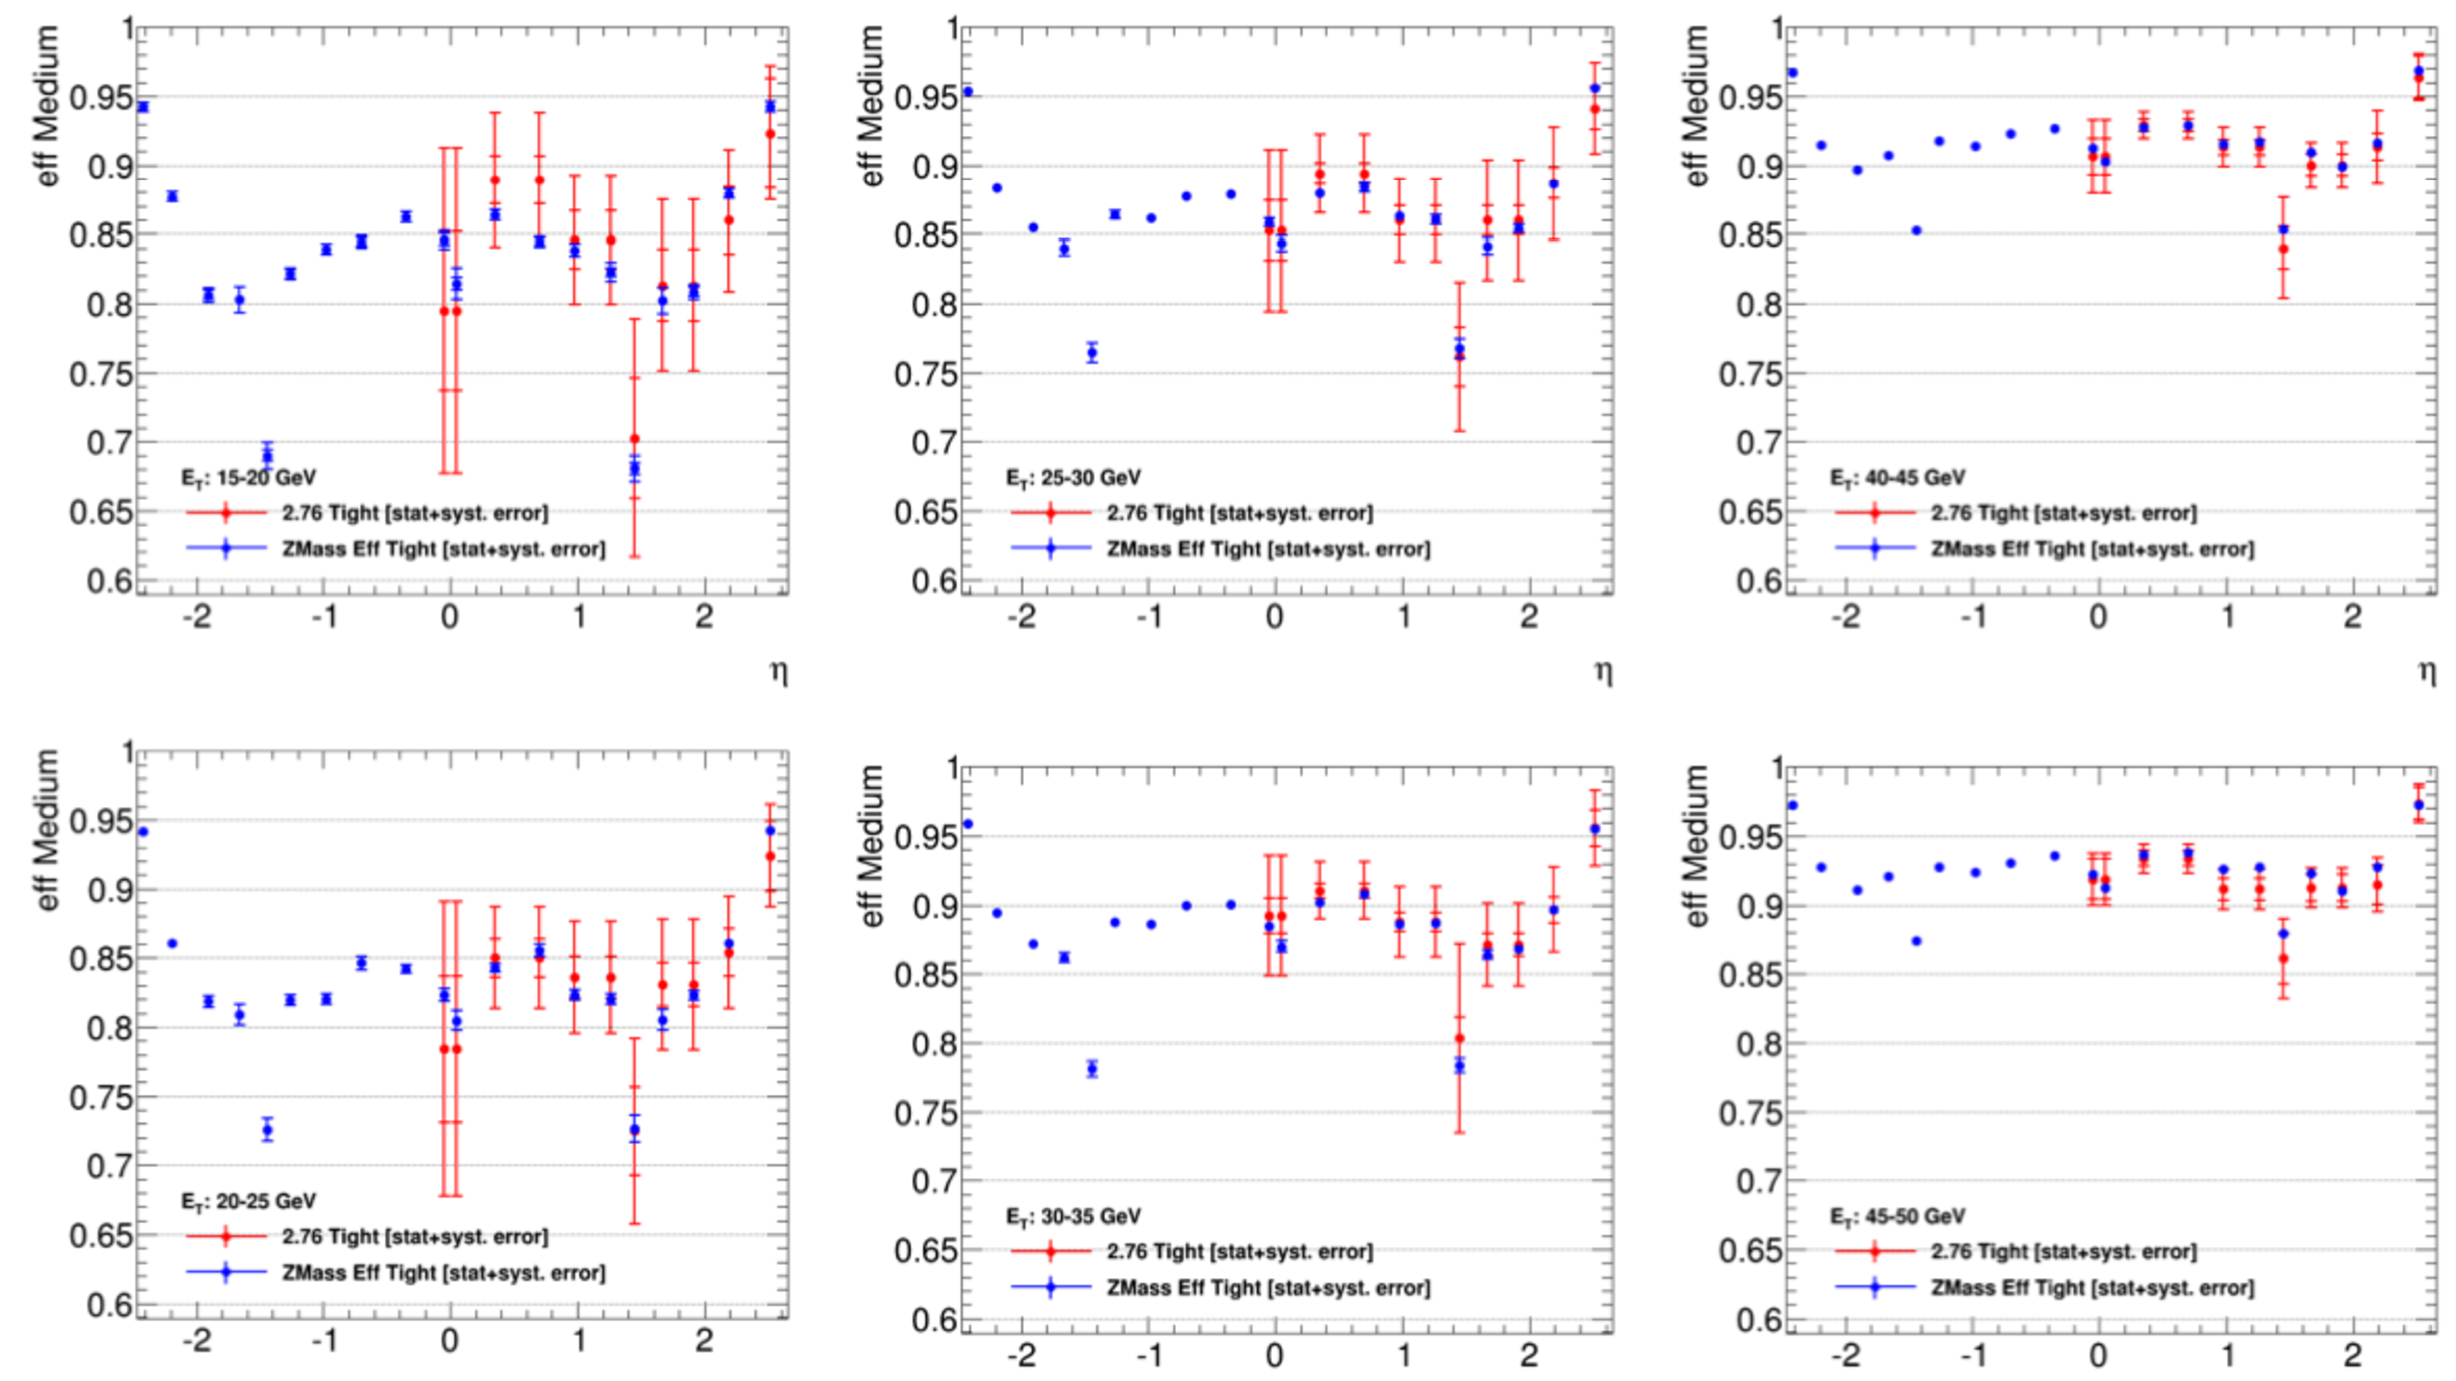
\includegraphics[width=1\textwidth]{MCCorrections/sf.pdf}
\caption{Comparition of electron efficiencies as calculated for 8TeV (blue points) and 2.76TeV (red points) for MC simulation. Efficiencies are shown as a function of pseudorapidity ($\eta$) for different electron $E_T$ bins. Both statistical and systematic uncertainties are shown. }
\label{eff_comp}
\end{figure}

Unfortunatelly, single muon trigger haven't been presented in a 2012 data, so muon trigger scale factor is calculated as a single number in order to minimize systematics contribution. 
\section{Electron energy scale and resolution}
Electrons clusters tend to shift in a reconstructed energy compared to a truth energy of initial electron. Correction of this shift is done on a both data and MC as a 3 step process:
\begin{itemize}
\item Electronic calibration, that transfers a raw signal from a readout to a cluster energy deposit.
\item MC based calibration. It corrects effects of energy loss in the material in front of calorimeter and leakage into the hadronic calorimeter. This calibration is applied on both data and MC.
\item Correction of calorimeter cell responce in data. This is allowing to get right responce in non-optimal HV-regions and exclude biases in a calorimeter electronics reconstruction.
\end{itemize}

Energy shift is parameterised, as:
\begin{equation}
E^{data}=E^{MC}(1+\alpha_i),
\end{equation}
where $E^{data}$ and $E^{MC}$ are the energies in data and simulation, respectivelly and $\alpha_i$ is a mean shift in a given bin i in $\eta$. 
Electron resolution is desribed by a formula \ref{eq:EMResoultion}. It is assumed, that sampling and noise terms are moddeled well by MC and the main diiference is coming from a constant term. 
The electron resoultion correction then can be written as:
\begin{equation}
\frac{\sigma_E}{E}^{Data}_{i}=\frac{\sigma_E}{E}^{MC}_{i} \oplus c_i
\end{equation}
where $c_i$ is $\eta$ dependent relative resolution correction. Parameters
$\alpha_i$ and $c_i$ are obtained from $Z\to ee$ invariant mass distribution with pseudorapidity configuration $(\eta_i, \eta_j)$ using $\chi^2$ fit. Resulting energy scale is applied on a data, while resolution is corrected for MC.

\section{Muon momentum correction}
\begin{equation}
\frac{\sigma_{ID}(p_T)}{p_T}=a_{ID}(\eta) \oplus b_{ID}(\eta) \cdot p_T
\end{equation}
\begin{equation}
\frac{\sigma_{MS}(p_T)}{p_T}=a_{MS}(\eta, \phi) \oplus b_{MS} (\eta, \phi) \cdot p_T \oplus \frac{c(\eta, \phi)}{p_T}
\end{equation}

\section{Hadron recoil correction}
